\documentclass{article}
\setlength{\parskip}{5pt} % esp. entre parrafos
\setlength{\parindent}{0pt} % esp. al inicio de un parrafo
\usepackage{amsmath} % mates
\usepackage[sort&compress,numbers]{natbib} % referencias
\usepackage{url} % que las URLs se vean lindos
\usepackage[top=25mm,left=20mm,right=20mm,bottom=25mm]{geometry} % margenes
\usepackage{hyperref} % ligas de URLs
\usepackage{graphicx} % poner figuras
\usepackage[spanish]{babel} % otros idiomas
\usepackage[utf8]{inputenc} % alparecer son los acentos
\documentclass[12pt,letterpaper]{article}
\usepackage[utf8]{inputenc}
\usepackage{tikz}
\usetikzlibrary{trees}
\usepackage[spanish, es-nodecimaldot]{babel}
\usepackage{color}
\usepackage{algorithm}
\usepackage[noend]{algpseudocode}
\renewcommand{\algorithmicrequire}{\textbf{Entrada:}}
\renewcommand{\algorithmicensure}{\textbf{Salida:}}
\usepackage{subcaption}
\usepackage{amsfonts}
\usepackage{hyperref}
 \hypersetup{
     colorlinks=true,
     linkcolor=blue,
     filecolor=blue,
     citecolor = blue,      
     urlcolor=cyan,
     }
\usepackage{amssymb}
\usepackage{listings}
\usepackage{color}
\author{I E G} % author
\title{Práctica 12 : red neuronal} % titulo
\date{\today}

\begin{document} % inicia contenido

\maketitle % cabecera

\begin{abstract} % resumen

En esta práctica se demuestra de forma básica el aprendizaje de una maquina donde reconoce dígitos de imágenes representadas en celdas pequeñas en blanco y negro con una red neuronal.
El elemento básico de una red neuronal es un perceptrón figura \ref{fig1} que esencialmente es un híperplano \cite{elis12} que busca colocarse en la frontera que separa las entradas verdaderas y las entradas falsas como en la \href{https://github.com/IsaacEstrada159/simulacion/blob/master/p12/p12p.gif}{animación}. Para efectos de esta práctica se estudia sistemáticamente el desempeño de la red neuronal en términos de su puntaje F para los diez dígitos $\{0, 1, 2, \ldots, 9\}$ en función de sus tres probabilidades asignadas a la generación de dígitos.



\begin{figure} [h!]% figura
    \centering
    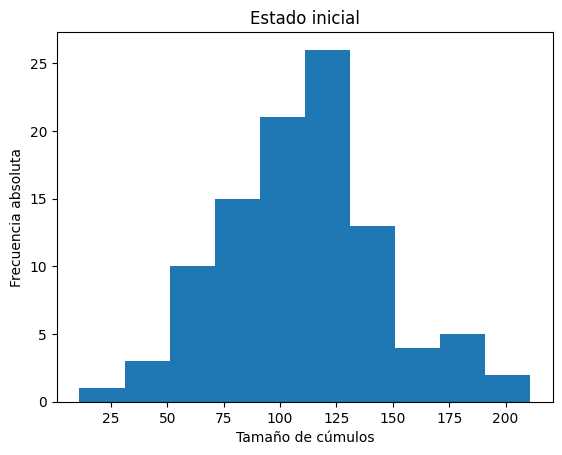
\includegraphics[width=129mm]{fig1.png} % archivo
    \caption{Prerceptrón.}
    \label{fig1}
\end{figure}

\end{abstract}


\section{Desarrollo}
Se utiliza el lenguaje de programación Python versión 3.9.6 para la generación del código previamente reportado en \cite{elis12} se utiliza también la herramienta de paralelización para que el código se ejecute con cuatro núcleos y se varían las probabilidades de generación de los dígitos, se suman los elementos no identificados y por ultimo se grafica en cajas – bigote los resultados de siete criterios con réplicas de 25 unidades.



  

\section{Experimento}
Para los diferentes criterios se grafica con diagramas caja – bigote donde se observa como la red neuronal realiza el funcionamiento y conforme se varia de forma negativa la probabilidad de generación de códigos la sumatoria de dígitos negados aumenta como en la figura \ref{fig2}.
\begin{figure} [h!]% figura
    \centering
    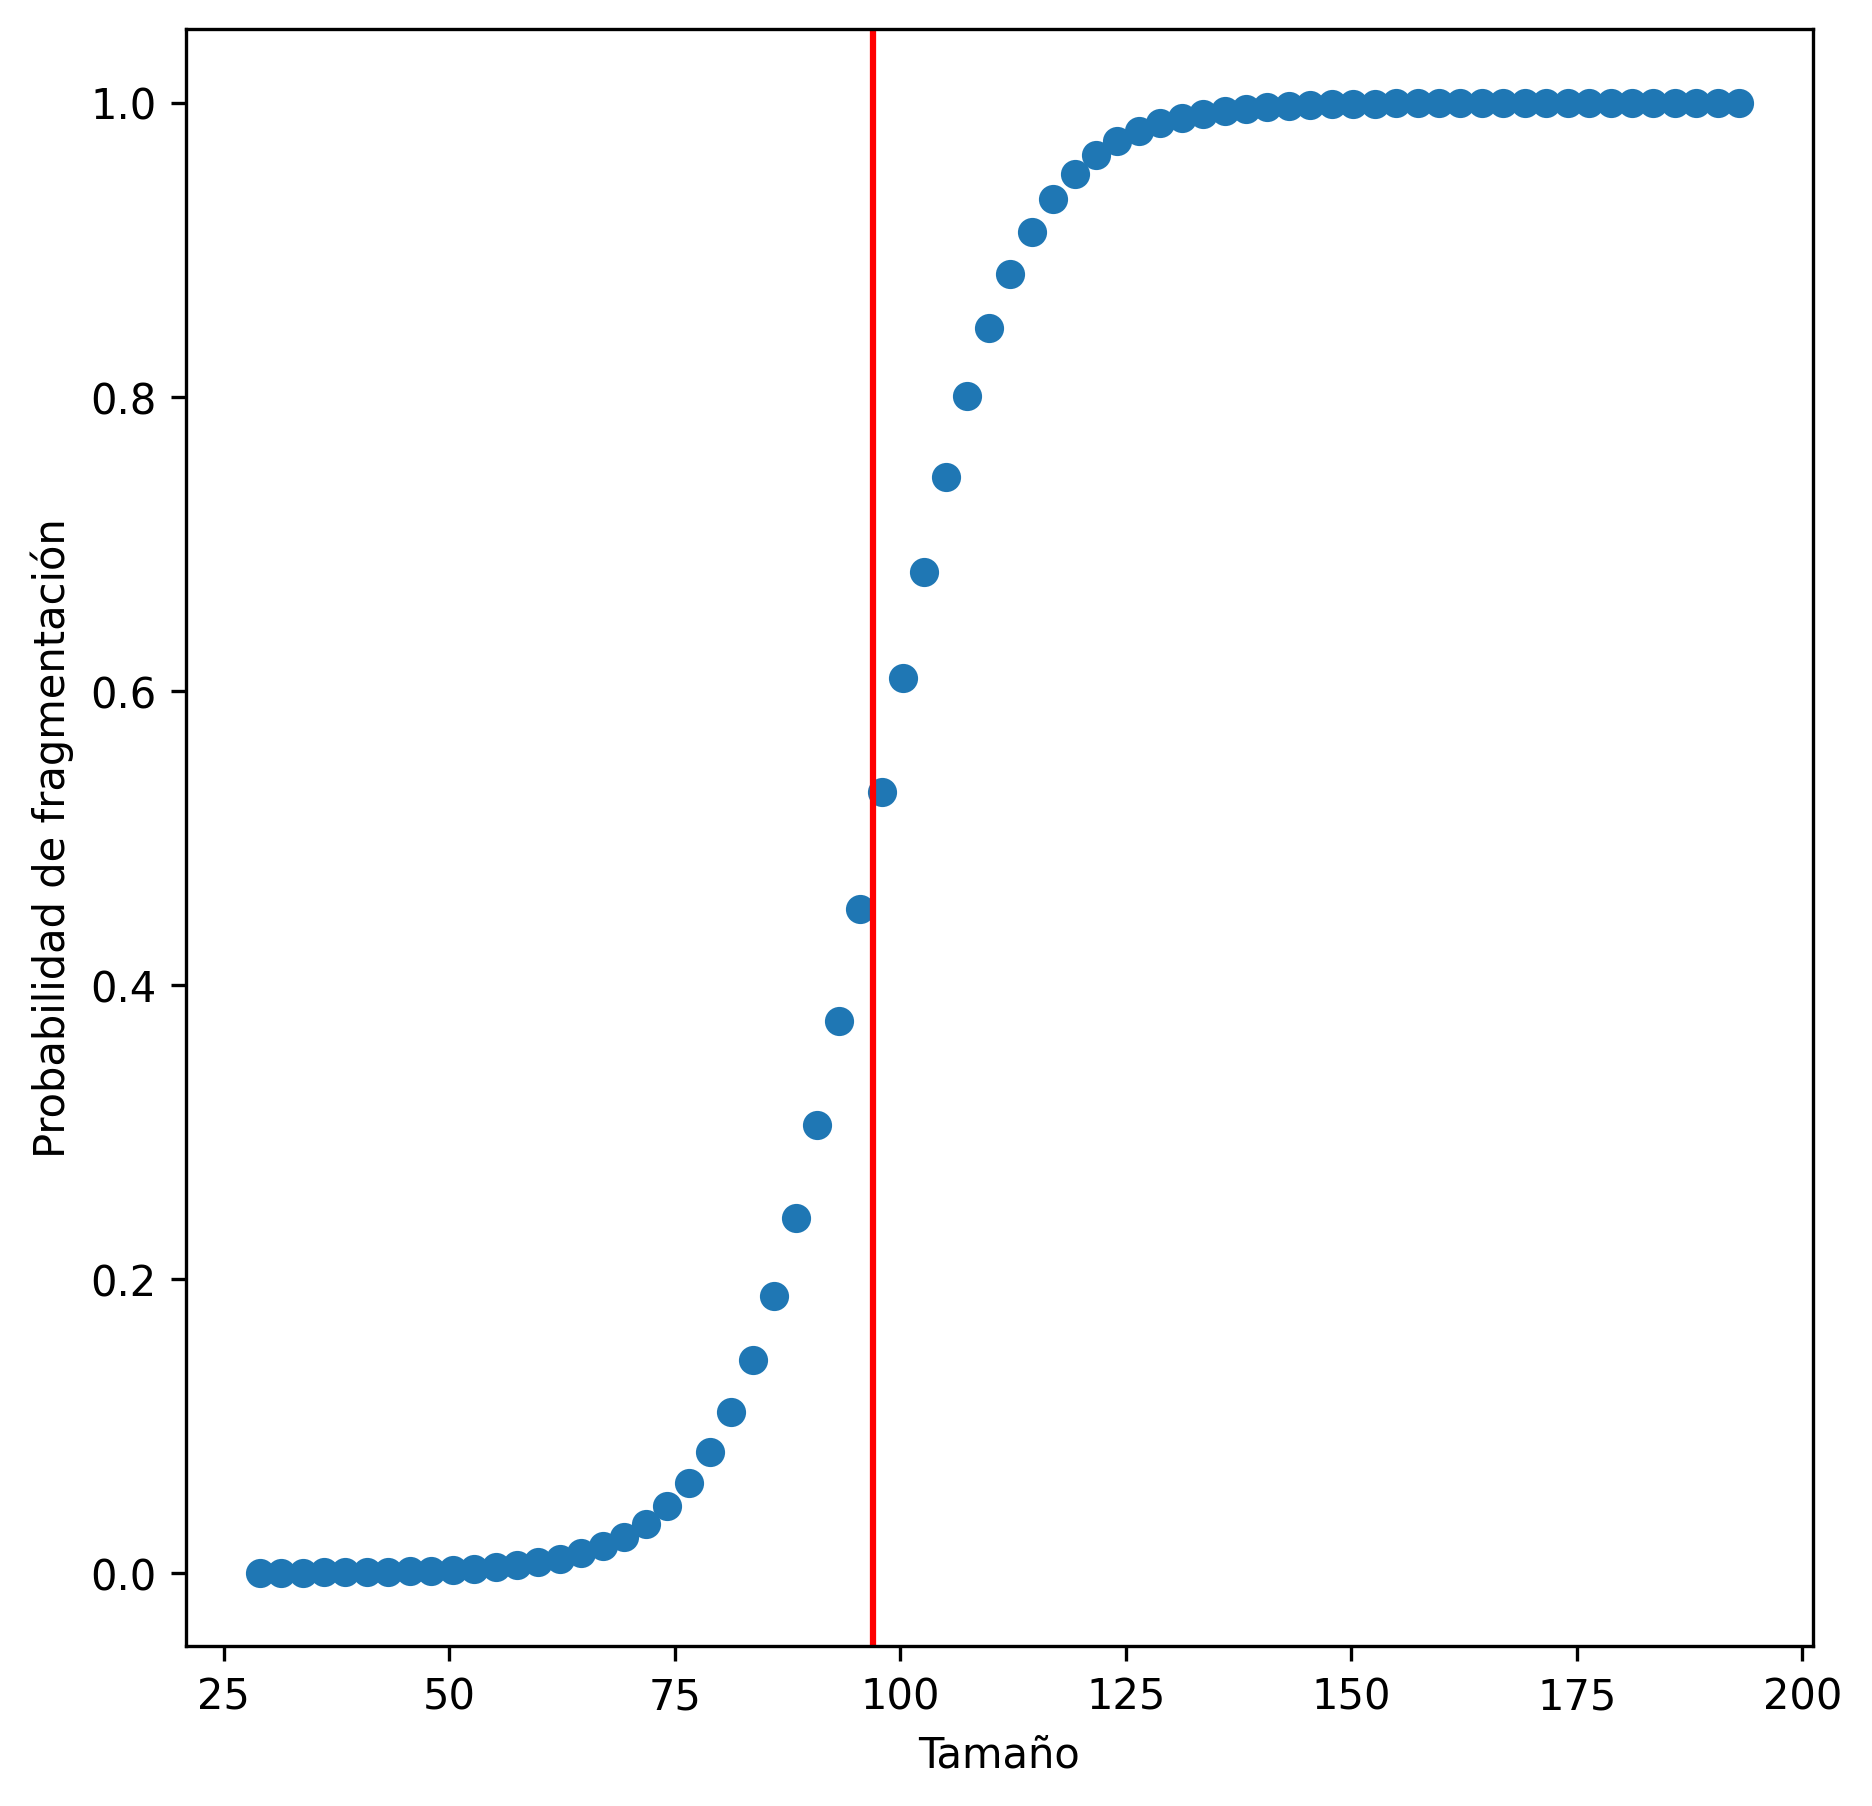
\includegraphics[width=85mm]{fig2.png} % archivo
    \caption{Gráficos de violín del porcentajes frente de Pareto.}
    \label{fig2}
\end{figure}


 
\section{Conclusiones} 

En conclusión, no se logro obtener el factor F pero se observo el funcionamiento de la red neuronal así como uno de los factores fundamentales como los números negados con los diferentes criterios y se observa cómo van aumentando debido a que la red no reconoce los dígitos.


\bibliography{bib}
\bibliographystyle{plainnat}

\end{document}